\section{Démarche Expérimentale}

\paragraph*{Calorimétrie}
Afin de déterminer le pouvoir calorifique des combustibles le montage à la \autoref{fig:montage} est utilisé. Le calorimetre échangeur de chaleur est un appareil permettant de mesurer les échanges de chaleur entre deux fluides, sans pertes. Lors de cette expérience, la combustion entraine une augmentation de l'énergie interne du calorimetre \(\Delta U_1\) ainsi qu'une augmentation de l'énergie interne de l'eau \(\Delta U_2\). La chaleur \(\mathcal{Q}\) produite par la combustion est donnée par la somme de la variation ces deux énergie internes, puisqu'aucun travail n'est effectué.
\begin{equation}
    \mathcal{Q} = \Delta U_1 + \Delta U_2
\end{equation}
Un état d'équilibre est atteint lorsque la différence entre la température d'entrée \(T_1\) et la température de sortie \(T_2\) de l'eau reste constante. Il n'y a alors plus d'augmentation de l'énergie interne du calorimètre, c'est à dire que \(\Delta U_1 = 0\).

\begin{figure}[h]
    \centering
    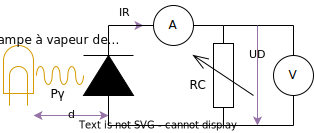
\includegraphics[width=0.7\linewidth]{figures/montage.png}
    \caption{Montage expérimental \cite{rapport-mendels-pascaud}}
    \label{fig:montage}
\end{figure}

\paragraph*{Pouvoir calorifique}
Afin de mesurer le pouvoir calorifique des combustibles, un brûleur contenant le combustible à étudier est allumé, chauffant le calorimètre. La combustion est considérée comme complète, puisqu'il y a un apport d'\ce{O2} suffisant à la flamme qui est en contact direct avec l'air ambiant. Les mesures s'effectuent lorsque l'état d'équilibre est atteint. La masse d'eau \(\Delta M\) est celle évacuée durant le temps pour consommer une certaine masse de combustible \(\Delta m\), celles-ci sont mesurées à l'aide de balances digitales. L'écart de température entre l'entrée d'eau et la sortie est relevé à l'aide de thermomètres. De plus, un bécher permet de récupérer l'eau de condensation produite au long de l'expérience. La masse d'eau condensée \(\Delta M_c\) est mesurée à la fin des mesures et divisée également sur toutes les mesures, cette approximation est faite en raison des faibles quantités considérées. Le pouvoir calorifique du combustible est alors donné par la différence entre l'énergie \(\Delta U_2\) reçue par l'eau qui circule et l'énergie de condensation de l'eau qui vient se rajouter à l'énergie de la combustion, tout ceci pris pour une masse de combustible brulé.
\begin{equation}
    H = \frac{\Delta U_2 - \Delta M_c \ell_\textrm{vap}^*}{\Delta m} = \frac{c^* \Delta M (T_2 - T_1) - \Delta M_c \ell_\textrm{vap}^*}{\Delta m}
    \label{eq:pouvoir_calorifique}
\end{equation}
avec \(c^* = (4179.6 \pm 0.1)\) \si{\joule\per\kelvin\per\kilo\gram} la capacité thermique massique de l'eau \cite{capacite-eau} et \mbox{\(\ell_\textrm{vap}^* = 2257\) \si{\kilo\joule\per\kilo\gram}} la chaleur latente massique de vaporisation de l'eau \cite{notice}.


\paragraph*{Ecart théorique-expérimental}
Afin de comparer les valeurs théoriques \(H_\textrm{théo}\) et expérimentales \(\langle H_\textrm{exp} \rangle\) obtenues dans le but d'estimer la fiabilité du montage et des résultats, l'écart relatif \(a\) est utilisé:
\begin{equation}
    a = \frac{ |H_\textrm{théo} - \langle H_\textrm{exp} \rangle| }{ H_\textrm{théo} }
    \label{eq:ecart_rel}
\end{equation}

\paragraph*{Détermination de la quantité de \ce{CO2} produit}
Afin de mieux comparer les combustibles, la quantité de \ce{CO2} produite est calculée expérimentalement à l'aide de la formule:
\begin{equation}
    m_{CO2} = \frac{\nu_{CO2}}{\nu_\textrm{combustible}} \frac{\Delta m}{M_\textrm{combustible}}M_{CO2}
    \label{eq:masse_co2}
\end{equation}
où \(M_\textrm{combustible}\) et \(M_{CO2}\) sont les masses molaires du combustible et du \ce{CO2} respectivement.
